\documentclass{article}
\usepackage{geometry,tikz}
\usetikzlibrary{calc,fit}
\geometry{paperwidth=52cm, paperheight=10cm,left=2pt,right=2pt,top=2pt,bottom=2pt}
\pagestyle{empty}
\setlength{\parindent}{0pt}
\tikzset{%
ref/.style={rounded corners=5mm,red},
der/.style={rounded corners,black,stealth-,densely dotted},
templ/.style={rounded corners,blue,-stealth},
point/.style={rounded corners,violet,-stealth,double}
}
\pgfdeclarelayer{background}
\pgfsetlayers{background,main}
\newcommand{\obj}[2][\relax]{\ifx#1\relax\texttt{#2<CoeffType>}\else\texttt{#1<CoeffType,#1>}\fi}
\begin{document}
\centering
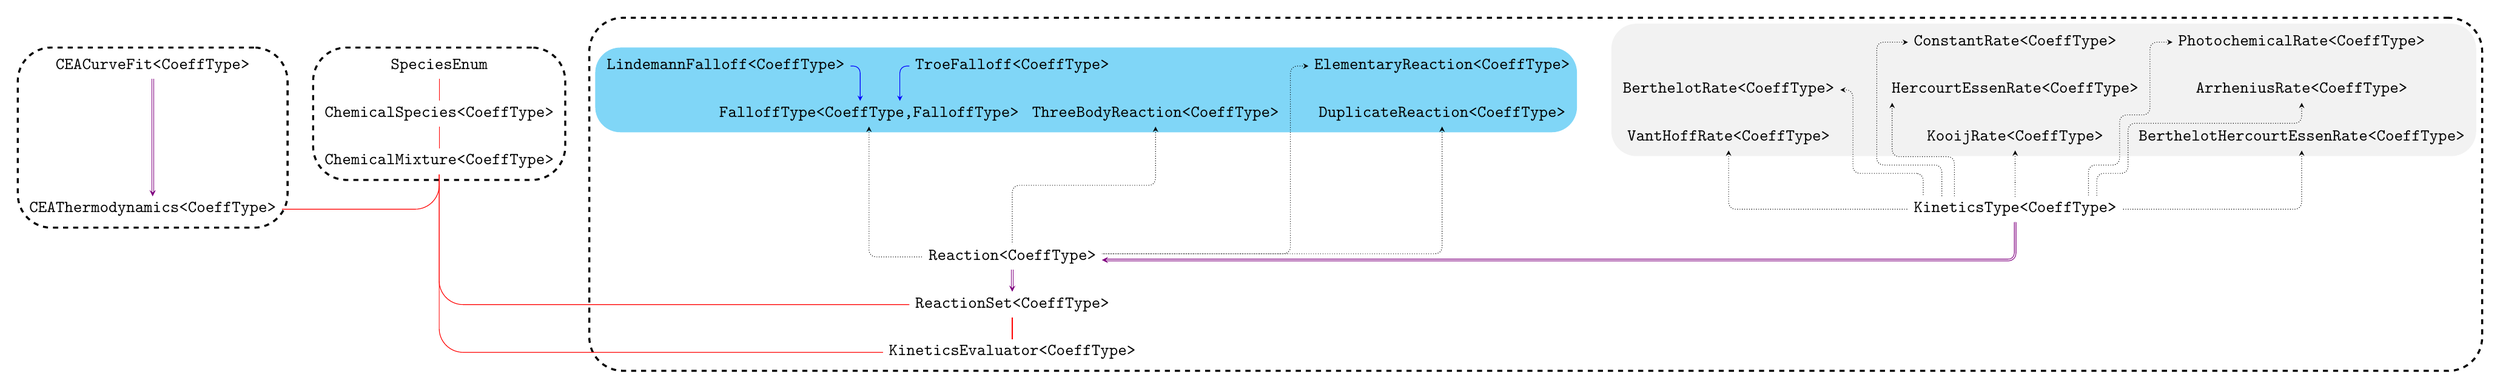
\begin{tikzpicture}[x=6cm,y=1cm,
                    every node/.append style={baseline}]
\node (SpecEnum) at (-7.5,1)  {\texttt{SpeciesEnum}};
%%
\node (ChemSpec) at (-7.5,0)  {\obj{ChemicalSpecies}};
\node (ChemMix)  at (-7.5,-1) {\obj{ChemicalMixture}};
%%
\node (CEAcurve)  at (-8.5,1)   {\obj{CEACurveFit}};
\node (CEAthermo) at (-8.5,-2)  {\obj{CEAThermodynamics}};
%%
%\node (LenJon)   at (-8.5,1)  {\obj{LennardJonesPotential}};
%\node (TranSpec) at (-8.5,0)  {\obj{TransportSpecies}};
%\node (TranMix)  at (-8.5,-2) {\obj{TransportMixture}};
%%
\foreach \kinMod/\modName/\i/\j in {ConstantRate/Con/-2/1.5,
                                    PhotochemicalRate/hv/-1/1.5,
                                    ArrheniusRate/Arr/-1/0.5,
                                    HercourtEssenRate/HE/-2/0.5,
                                    BerthelotRate/B/-3/0.5,
                                    BerthelotHercourtEssenRate/BHE/-1/-0.5,
                                    KooijRate/Kooij/-2/-0.5,
                                    VantHoffRate/VH/-3/-0.5%
                                   }
     \node (\modName)      at (\i,\j) {\obj{\kinMod}};
\node (KinMod) at (-2,-2) {\obj{KineticsType}};
%%
\foreach \fall/\name/\i in {LindemannFalloff/Lin/-6.5,TroeFalloff/Troe/-5.5}
     \node (\name)   at (\i,1) {\obj{\fall}};
%%
\foreach \ChemPro/\modName/\i/\j in {ElementaryReaction/Elem/-4/1,
                                  DuplicateReaction/Dupl/-4/0,
                                  ThreeBodyReaction/TB/-5/0%
                                   }
     \node (\modName)      at (\i,\j) {\obj{\ChemPro}};
\node (FO)      at (-6,0) {\obj[FalloffType]{FalloffReaction}};
%%
\node (reaction)    at (-5.5,-3) {\obj{Reaction}};
\node (reactionSet) at (-5.5,-4) {\obj{ReactionSet}};
\node (kinEval)     at (-5.5,-5) {\obj{KineticsEvaluator}};
%%%%%%%%%%%%%%
%%%%%%%%%%%%%%
%%
\draw[ref] (SpecEnum) -- (ChemSpec);
%\draw[ref,rounded corners=5pt] (SpecEnum) -| ($(TranSpec)!0.55!(SpecEnum)$) |- (TranSpec);
%%
\draw[ref] (ChemSpec) -- (ChemMix);
%
\draw[point] (CEAcurve) -- (CEAthermo);
\draw[ref]   (ChemMix)  |- (CEAthermo);
%
%\draw[ref] (LenJon)   -- (TranSpec);
%\draw[ref] (TranSpec) -- (TranMix);
%\draw[ref] (ChemMix)  |- (TranMix);
%%
\draw[der] (Con)   -| ($(B.east)!0.8!(HE.west)$) |- ([yshift=5pt]$([xshift=-5pt]Kooij.west)!0.5!(KinMod.west)$) -| (KinMod.170);
\draw[der] (hv)    -| ([yshift=5pt]$(Arr.west)!0.7!(BHE.west)$) 
                   -| ([xshift=-5pt]$(BHE.west)!0.2!(Kooij.east)$) |- ([yshift=5pt,xshift=-5pt]$(Kooij.east)!0.5!(KinMod.east)$) 
                   -| (KinMod.10);
\draw[der] (Arr)   |- ($(Arr.west)!0.7!(BHE.west)$)  -| ($(BHE.west)!0.2!(Kooij.east)$) |- ($(Kooij.east)!0.5!(KinMod.east)$) -| (KinMod.9);
\draw[der] (HE.186) |- ([yshift=10pt]$([xshift=-5pt]Kooij.west)!0.5!(KinMod.west)$) -| (KinMod.168);
\draw[der] (B)     -| ($(VH.east)!0.2!(Kooij.west)$) |- ($([xshift=-5pt]Kooij.west)!0.5!(KinMod.west)$) -| (KinMod.172);
\draw[der] (BHE)   |- (KinMod);
\draw[der] (Kooij) -- (KinMod);
\draw[der] (VH)    |- (KinMod);
%%
\draw[templ] (Lin.east)  -| ([xshift=2mm]Lin.east |- FO.north);
\draw[templ] (Troe.west) -| ([xshift=-2mm]Troe.west |- FO.north);
%%
\draw[der] (Elem) -| ($(Dupl.west)!0.8!(TB.east)$) |- (reaction.2);
\draw[der] (Dupl) |- (reaction.2);
\draw[der] (TB)   |- ($(TB)!0.5!(reaction)$)   -| (reaction);
\draw[der] (FO)   |- (reaction);
%%
\draw[point] (KinMod) |- (reaction.-2);
%%
\draw[point] (reaction) -- (reactionSet);
\draw[ref]   (ChemMix)  |- (reactionSet);
\draw[ref]   (ChemMix)  |- (kinEval);
\draw[ref]   (reactionSet) -- (kinEval);
%%%
\begin{pgfonlayer}{background}
\node[fit= (hv) (B) (BHE), fill = gray!10, rounded corners=15pt ] (kin) {};
\node[fit= (Lin) (Dupl), fill = cyan!50, rounded corners=15pt ] (chem) {};
\node[draw, fit = (chem) (kin) (kinEval), rounded corners=20pt, dashed, very thick] {};
\node[draw, fit = (SpecEnum) (ChemSpec) (ChemMix), rounded corners=20pt, dashed, very thick] {};
\node[draw, fit = (CEAcurve) (CEAthermo), rounded corners=20pt, dashed, very thick] {};
\end{pgfonlayer}
\end{tikzpicture}
\end{document}
